\documentclass{article}

\usepackage[utf8]{inputenc}
\usepackage[ngerman]{babel}
\usepackage[T1]{fontenc}
\usepackage{enumitem}
\usepackage{graphicx}
\usepackage{float}

\newlist{FA}{enumerate}{1}
\setlist[FA]{label=/FA\arabic*/}

\newlist{NA}{enumerate}{1}
\setlist[NA]{label=/NA\arabic*/}


\title{Cryptographics Pflichtenheft}
\author{}
\date{\today}

\begin{document}

\maketitle
\tableofcontents
\newpage

\section{Zielbestimmung}


Im Rahmen der PSE-Veranstaltung soll für das Kryptologikum des Instituts für 
Kryptographie und Sicherheit eine Software (Cryptographics / Anicrypto?) zur 
Demonstration kryptographischer Verfahren erstellt werden. \\
\\
Das Programm soll im Laufe der Ausstellung Kryptologikum das Interesse der Besucher wecken, sich mit Verschlüsselung zu befassen und schließlich auch ausgewählte Inhalte der Kryptographie näher bringen. \\
\\
Wichtig ist, dass die Visualisierungen ansprechend und verständlich gestaltet sind. Die Nutzung von Cryptographics soll Spaß machen. \\
\\
Jedes Verfahren wird hierbei in drei Schritten vorgestellt. Diese sind eine Demo, ein interaktiver Versuch und ein wiki-artiger Artikel für weitere Informationen.
In der Demo wird dem Nutzer der Ablauf der Verschlüsselung möglichst anschaulich demonstriert. Darauf folgend kann im Eigenversuch auf der gleichen Oberfläche die Verschlüsselung selbst ausprobiert werden. Dem Nutzer wird hierbei eine größtmögliche Freiheit zur Wahl sämtlicher Komponenten (wie Klartext, Primzahl, etc.) gelassen. Unter "Mehr Wissen" sollen sich interessierte Benutzer schließlich tiefgehender über das Verfahren informieren können, über seine Entstehung, Einsatz und Nachfolger. Auf geeignete weiterführende Literatur kann mit QR-Codes verwiesen werden. \\


\subsection{Musskriterien}

\begin{itemize}
    \item Visualisierung Caesar-Chiffre
    \item Visualisierung Vigenère-Chiffre
    \item Visualisierung Diffie-Hellmann
    \item Robuste Programmierung
    \item Intuitive Benutzerführung
    \item Schnelle Reaktionszeiten
    \item Zugriff auf Krypto-Verfahren über Zeitleiste
    \item Benutzerführung über Phasen
    \item Angeleiter Selbstversuch bei komplexen Verfahren
    \item Interaktion des Benutzers über den Touchscreen
    \item einfache, übersichtliche UI, die sich gut auf Touchscreen bedienen lässt
    \item Robustheit gegen au"sergewöhnliche Interaktion
    \item Man soll das Programm nicht schlie"sen können währen der Vorführung
    \item Praxisbezug auf moderne Kryptoverfahren
    \item Eingängige optische Darstellung der verschiedenen Verfahren
    \item Krypto-Algorithmen lassen sich schrittweise ausführen, um den Prozess
        langsam zu verdeutlichen
    \item Beenden des Programms / Wechsel zum Desktop nur per angeschlossener Tastatur, nicht über Touch-Eingabe
    \item Das Programm darf zu keinem Zeitpunkt in einen undefinierten Zustand fallen
    \item Es darf nicht möglich sein das Programm in eine Sackgasse zu führen, die einen Neustart erfordert
    \item Time-Out bei fehlender Nutzerinteraktion, Rückkehr zum Startbildschirm
    \item Es ist jederzeit möglich über einen Button zurück zur Startoberfläche zu gelangen
\end{itemize}

\subsection{Wunschkriterien}

\begin{itemize}
    \item Visualisierung Public Key – Infrastruktur
    \item Visualisierung Shamir Secret Sharing
    \item Visualisierung Passwortsicherheit
    \item Visualisierung One-Time-Pad
    \item Visualisierung Blockchiffre (DES, AES)
    \item Visualisierung Hashfunktionen
    \item Visualisierung RSA
    \item Modulares Austauschen/Hinzufügen von weiteren kryptografischen Verfahren
    \item Literaturhinweise(auch weiterführende Literatur), sofern Interesse besteht.
    \item Visualisierungen sollten möglichst ansprechend sein, indem sie z.B. Analogien 
        verwenden (ein Datenpaket wird zu einer Postkarte, ein Schlüssel wird zum einem tatsächlichen Schlüssel, ...).
    \item Visualisierungen sollten Grafiken und Animationen verwenden um Vorgänge zu verdeutlichen
    \item Visualisierung von Angriffen auf Verfahren
    \item Erfassung von Nutzungsstatistiken
    \item Animation auf Startbildschirm
\end{itemize}

\subsection{Abgrenzungskriterien}
\begin{itemize}
    \item Sämtliche kryptologischen Verfahren werden nur zu Vorführungszwecken implementiert. Eine sichere Implementierung ist nicht vorgesehen.
    \item Dies ist ein Vorführprogramm für eine Ausstellung, demnach ist eine andere  Verwendung nicht ratsam, 
        da dafür ganz andere Anforderungen gelten, die hier nicht beachtet werden. (umformulieren!)
    \item keine optimierte und 100\% standardkonforme Implementierung von Krypto-Algorithmen, 
        sondern Fokus auf schrittweiser Ausführbarkeit
    \item keine formale Korrektheit bei Erklärungen sondern Ansatz ohne nötige Vorkenntnisse 
        um breiter Masse zugänglich zu sein
    \item nicht zur tatsächlichen Verschlüsselung von Texten gedacht 
\end{itemize}

\section{Produkteinsatz}
\subsection{Anwendungsbereiche}
Cryptographics soll in erster Linie als Ausstellungsstück für das Kryptologikum des Instituts für Kryptographie und Sicherheit (IKS) am Karlsruher Institut für Technologie (KIT) dienen. 

Besuchern der Ausstellung soll das Funktionsprinzip und die Verwendung historischer, sowie aktueller, kryptographischer Verfahren nähergebracht werden. Diese sollen anhand von vereinfachten und beispielhaften Szenarien aus dem Alltag vermittelt werden, mit dem Ziel, ein größeres Interesse an der Materie zu wecken.

Cryptograhics soll primär auf dem eeePC (siehe Produktumgebung) im Kryptologikum eingesetzt werden. Portabilität wäre jedoch wünschenswert.

\subsection{Zielgruppen}

Das Programm richtet sich insbesondere an Kinder, Jugendliche und Erwachsene mit grundlegenden Kenntnissen der Mathematik. Die Zielgruppe ist demnach ein anonymes Publikum, das sich potenziell aus fachfremden Personen zusammensetzt. Deshalb dürfen für die Verwendung von Cryptographics keine Vorkenntnisse in der Kryptographie vorausgesetzt werden.

\subsection{Betriebsbedingungen}

Das Programm soll im Dauerbetrieb problemlos laufen. Dementsprechend dürfen keine Ausnahmen auftreten, die den Betrieb des Programms behindern, oder gar einen Absturz auslösen, der den Benutzer zur Betriebssystemebene führt. Insbesondere muss darauf geachtet werden, dass schnelle, unkontrollierte Benutzereingaben zu keinem undefinierten Zustand des Programms führen. Auch ein reguläres Beenden von Cryptographics soll durch den Benutzer nicht möglich sein, und nur durch eine angeschlossene Hardwaretastatur erreicht werden können.

Der Betrieb soll für die Hardware des eeePC (siehe Produktumgebung) optimiert sein, der während der Ausstellung über keine Internetverbindung verfügt. Inhalte zu weiterführenden Informationen müssen also lokal in Form von leicht aktualisierbaren und austauschbaren Textdateien vorliegen.

\section{Produktumgebung}

Software/Hardware… => Weiß ich grad nicht. XP auf nem eeePc
Einsatz auf eeePC wieauchimmer (keine Ahnung wie die Kiste heißt)
- Produktumgebung ist ein Windows-PC mit reisistivem Touchscreen 
und Windows XP

\subsection{Software}

\subsection{Hardware}

\section{Produktfunktionen}

\subsection{Funktionale Anforderungen}

\subsubsection{Grundfunktionen}

\begin{FA}[start=100]
\item Darstellung aller Visualisierungen auf einer Zeitleiste
\item Interaktion mit der Zeitleiste, um eine einzelne Visualisierung auswählen zu können
\item Darstellung einer Übersichtsseite zur gewählten Visualisierung
\item Start der gewählten Visualisierung
\item Abbruch einer gewählten Visualisierung, um zum Startbildschirm zurückzukehren
\item Darstellung weiterführender Information nach erfolgreichem Beenden einer Visualisierung
\end{FA}

% TODO: do we really need/want this?
%/FA200/ Erfassen von Nutzungsdaten zur Optimierung des Ausstellungsstückes durch
%/FA201/ - Abbruchquote einer Visualiserung
%/FA202/ - Anzahl Starts einer Visualiserung
%/FA203/ - Bearbeitungsdauer einer Visualisierung
%/FA204/ - Gesamtlaufzeit des Programmes
%/FA205/ - Idle-Zeit des Programmes
%/FA206/ - Fehlversuche beim Lösen einer Herausforderung

\begin{FA}[start=100]
\item Prozess: Diffie-Hellman Schlüsselaustausch Demonstration
\end{FA}
\begin{itemize}[label={}]
    \item Ziel: Vermittlung des Diffie-Hellman Schlüsselaustauschs mit Farben-Analogie
    \item Vorbedingung: keine
    \item Nachbedingung (Erfolg): Alice und Bob haben sich auf eine
        gemeinsame, geheime Farbe geeinigt die Eve nicht kennt
    \item Nachbedingung (Fehlschlag): Gibt es nicht, da nur
        eine Demonstration ausgeführt wird
    \item Auslösendes Ereignis: Ausgewählt in der Timeline
\end{itemize}

Beschreibung:
\begin{enumerate}
    \item Erkläre das Ziel sich auf ein gemeinsames Geheimnis zu einigen,
        durch Nutzung eines unsicheren Übertragungskanals
        bei dem Eve lauschen kann, ohne dass Eve das Geheimnis erfährt
    \item Demonstriere das Prinzip der Einwegfunktion, anhand Farben die man mischen
        kann. Farben zu mischen ist einfach, zur einer gemischten Farbe
        herauszufinden welche Farben verwendet wurden hingegen ist schwer
    \item Alice und Bob einigen sich auf eine gemeinsame, nicht geheime Farbe A
    \item Alice wählt eine geheime Farbe X und mischt sie mit A zur Farbe AX
    \item Bob wählt eine geheime Farbe Y und mischt sie mit A zur Farbe AY
    \item Alice schickt AX zu Bob u. Bob schickt AY zu Alice
    \item Alice mischt X mit AY zu AYX
    \item Bob mischt Y mit AX zu AXY
    \item Wenn Eve weder X noch Y erfahren hat, kennt Eve nicht AXY
\end{enumerate}

\begin{FA}[start=100]
\item Prozess: Diffie-Hellman Schlüsselaustausch Selbstversuch
\end{FA}
\begin{itemize}[label={}]
    \item Ziel: Der Nutzer hat einen erfolgreichen Diffie-Hellman Schlüsselaustausch
        (mit Farben-Analogie) mit Bob durchgeführt
    \item Vorbedingung: keine
    \item Nachbedingung (Erfolg): Alice und Bob haben sich auf eine
        gemeinsame, geheime Farbe geeinigt die Eve nicht kennt
    \item Nachbedingung (Fehlschlag): Alice und Bob haben eine gemeinsame,
        nicht geheime Farbe oder sich auf gar keine Farbe geeinigt
    \item Auslösendes Ereignis: Ende der Demonstration des Diffie-Hellman
        Schlüsselaustauschs mit Farben, oder die Demonstration wurde Übersprungen
\end{itemize}

Beschreibung:
\begin{enumerate}
    \item Der Nutzer übernimmt die Rolle von Alice
    \item Benenne die Aufgabe, dass der Nutzer (Alice) sich auf ein gemeinsames Geheimnis
        mit Bob einigt, wobei ein öffentlicher Kanal genutzt wird auf dem Eve lauscht,
        ohne dass Eve das Geheimnis erfährt.
    \item Der Nutzer (Alice) wird aufgefordert eine Farbe A zu wählen,
        wurde diese gewählt, wird der Nutzer aufgefordert
        die nicht geheime Farbe an Bob zu schicken.
    \item Der Nutzer soll nun eine geheime Farbe X != A wählen,
        diese soll er an Bob schicken
    \item Bob wählt eine geheime Farbe Y und mischt sie mit A zur Farbe AY
    \item Der Nutzer kann nun eine Farbe zu Bob schicken,
        wenn er die private Farbe X schickt hat er verloren,
        wenn er A schickt hat er ebenso verloren,
        wenn er AX schickt geht es weiter
    \item Der Nutzer wird aufgefordert nun die richtigen Farben zu mischen,
        wenn er X mit AY mischt geht es weiter, wenn nicht hat er verloren.
    \item Bob mischt Y mit AX zu AXY
    \item Wenn Eve weder X noch Y erfahren hat, kennt Eve nicht AXY,
        der Nutzer kann beglückwünscht werden
\end{enumerate}

\begin{FA}[start=200]
\item Kryptographische Verfahren auswählen
\end{FA}

\begin{FA}[start=300]
\item Funktionen von den jeweiligen Verfahren abhängig
\end{FA}

\begin{FA}[start=400]
\item Jederzeit die Möglichkeit für interaktive Hilfe ([?]-Button)
\end{FA}

\subsubsection{Erweiterte Funktionen}

\begin{FA}[start=500]
\item Public Key Infrastruktur (PKI)
\end{FA}
\begin{itemize}[label={}]
\item Prozess: Erläuterung der Vorgänge bei der Verteilung von öffentlichen Schlüsseln.
\item Ziel: Dem Benutzer ist klar ersichtlich, wie die Verteilung vonstatten geht und welche Instanzen in diesem Rahmen interagieren.
\item Akteure: Benutzer.
\item Beschreibung:
\item Phase 1: Animation.
\begin{enumerate}
\item Auf dem Bildschirm erscheinen Animationen, die die Verteilung veranschaulichen.
\item Der Benutzer sieht die Animation schrittweise und kann sie jederzeit anhalten, vorwärts oder rückwärts gehen.
\item An die Demo anschließend springt das Programm in die Phase 3, Wiki. 
\end{enumerate}
\item Phase 2: Selbstversuch. Wird übersprungen, da sich die Überlegungen zu einem Selbstversuch in PKI keine vernünftigen Ergebnisse liefern. Ein Selbstversuch kann aber jederzeit eingebaut werden.
\item Phase 3: Wiki.
\begin{enumerate}
\item Nach dem Durchlesen ist die Visualisierung des Public-key Infrastruktur abgeschlossen. Der Benuter wird zum nächsten Verfahren weitergeleitet.
\item //Todo(Mach ich noch heute abend oder morgen früh, da hierzu man bestimmt sehr schöne Erklärungen machen kann! Keine Lust jetzt was billiges hinzuklatschen. Auch die globalen Testfälle mache ich später.):
\end{enumerate}
\end{itemize}

\begin{FA}[start=500]
\item One Time Pad
\end{FA}

\begin{itemize}[label={}]
\item Prozess: Visualisierung des Verfahrens One Time Pad.
\item Ziel: Benutzer versteht das Verfahren und kann selbstständig beliebigen Klartext verschlüsseln und beliebigen Chiffrat, der mit dem One Time Pad erzeugt wurde, entschlüsseln.
\item Akteure: Benutzer.
\item Beschreibung:
\item Phase 1: Animation.
\begin{enumerate}
\item Erklärung des Verfahrens anhand von verschiedenen Animationen.
\item Der Benutzer kann die Animation schrittweise vollziehen und falls nötig schrittweise zurück gehen.
\item Am Ende der Animation wechselt die Visualisierung des Verfahrens in die zweite Phase, dem Selbstversuch.
\end{enumerate}

\item Phase2: Selbstversuch.
\item Schritt 1:
\begin{enumerate}
\item Vom Benutzer wird eine Eingabe getätitgt. Diese besteht aus dem Klartext, den es zu verschlüsseln gilt, sowie auch dem Schlüssel. Aus der vorherigen Demo sollte der Benutzer es verstanden haben, wie der Schlüssel auszusehen hat. Oder er lässt sich die Eingabe vom Programm generieren.
\item Die Funktionalen Anforderungen und der Aufbau des ersten Schrittes des Selbstversuches ist analog zum /F2/. Die Unterschiede sind logischer Natur, wie die Länge des Schlüssels zum Beispiel. Der Benutzer verschlüsselt also mit einem Vigenere, wobei die Schlüssellänge gleich der Länge des Klartextes ist.
\item Nachdem der Benutzer die Eingabe entsprechend verschlüsselt und das Programm das Chiffrat entschlüsselt und verglichen hat, wechselt im Falle des Erfolgs der Selbstversuch in Schritt 2.
\end{enumerate}

\item Schritt 2:
\begin{enumerate}
\item Die Funktionalen Anforderungen sind im Schritt 2 ebenfalls identisch zu /F2/. Chiffrat wird generiert und Benutzer entschlüsselt das Chiffrat mit einem gegebenen Schlüssel, wie ein Vigenere Chiffrat entschlüsseln würde.
\item Nachdem alles richtig entschlüsselt wurde und der Benutzer sich über sein neu gewonnenes Wissen freut wechselt die Visualisierung in die Phase 3, dem Wiki-Teil, wo der Benutzer sich noch mehr freuen kann.
\end{enumerate}

\item Phase3: Wiki.
\begin{enumerate}
\item Nach dem Durchlesen ist die Visualisierung von One Time Pad abgeschlossen. Der Benuter wird zum nächsten Verfahren weitergeleitet.
\end{enumerate}
\end{itemize}

- Funktionen: Willkommensbildschirm, Algo/Visualisierung wählen, Algo bearbeiten, 
Soforthilfe passend zum Algo falls man nicht weiter weiß, Algo beenden, 
ggf. Kontrollfragen oder selbstständiges Anwenden des Gelernten am Ende (z.B. ein Wort mit Caesar verschlüsseln)
\\
\\
RSA und Public-Key Verschlüsselung anhand von Pad-Locks als 
öffentliche Schlüssel und den Schlüssel  dazu als privaten,
vielleicht mit Komplementärfarben visualisieren ähnlich wie Diffie-Hellman



\subsection{Nichtfunktionale Anforderungen}

\begin{NA}[start=100]
\item Schnelle Reaktionszeit
\end{NA}
\begin{NA}[start=200]
\item Große Robustheit
\end{NA}
\begin{NA}[start=300]
\item Intuitive Benutzerführung
\end{NA}

- Die Anwendung muss möglichst performant und verzögerungsfrei auf Benutzereingaben reagieren (soweit das die HW zulässt...)
\\
\\
- Die Anwendung muss leicht zu bedienen sein

\section{Produktdaten}

\subsection{Nutzerdaten}

Zu speichern sind ggf. Nutzungsstatistiken, um herauszufinden, welche Visualisierung gut ankommt und welche nicht. 
Dies erlaubt das Ausstellungsstück zielgerichtet weiterzuentwickeln.

\section{Benutzerschnittstelle}

\subsection{Ablauf einer Visualisierung}

Der Willkommensbildschirm besteht einem einleitenden Text, der das Ausstellungsstück kurz dem Publikum vorstellt, und einer Zeitleiste (Fig. 1). Auf der Zeitleiste werden mithilfe einer geeigneten Skala Jahreszahlen dargestellt. Die kryptografischen Visualisierungen werden auf dieser Zeitleiste mithilfe von "Meilensteinen" dargestellt. Weiterhin werden die Markierungen in grün, gelb oder rot eingefärbt, um den Schwierigkeitsgrad auf einen Blick erkennbar zu machen.

\begin{figure}[H]
  \centering
    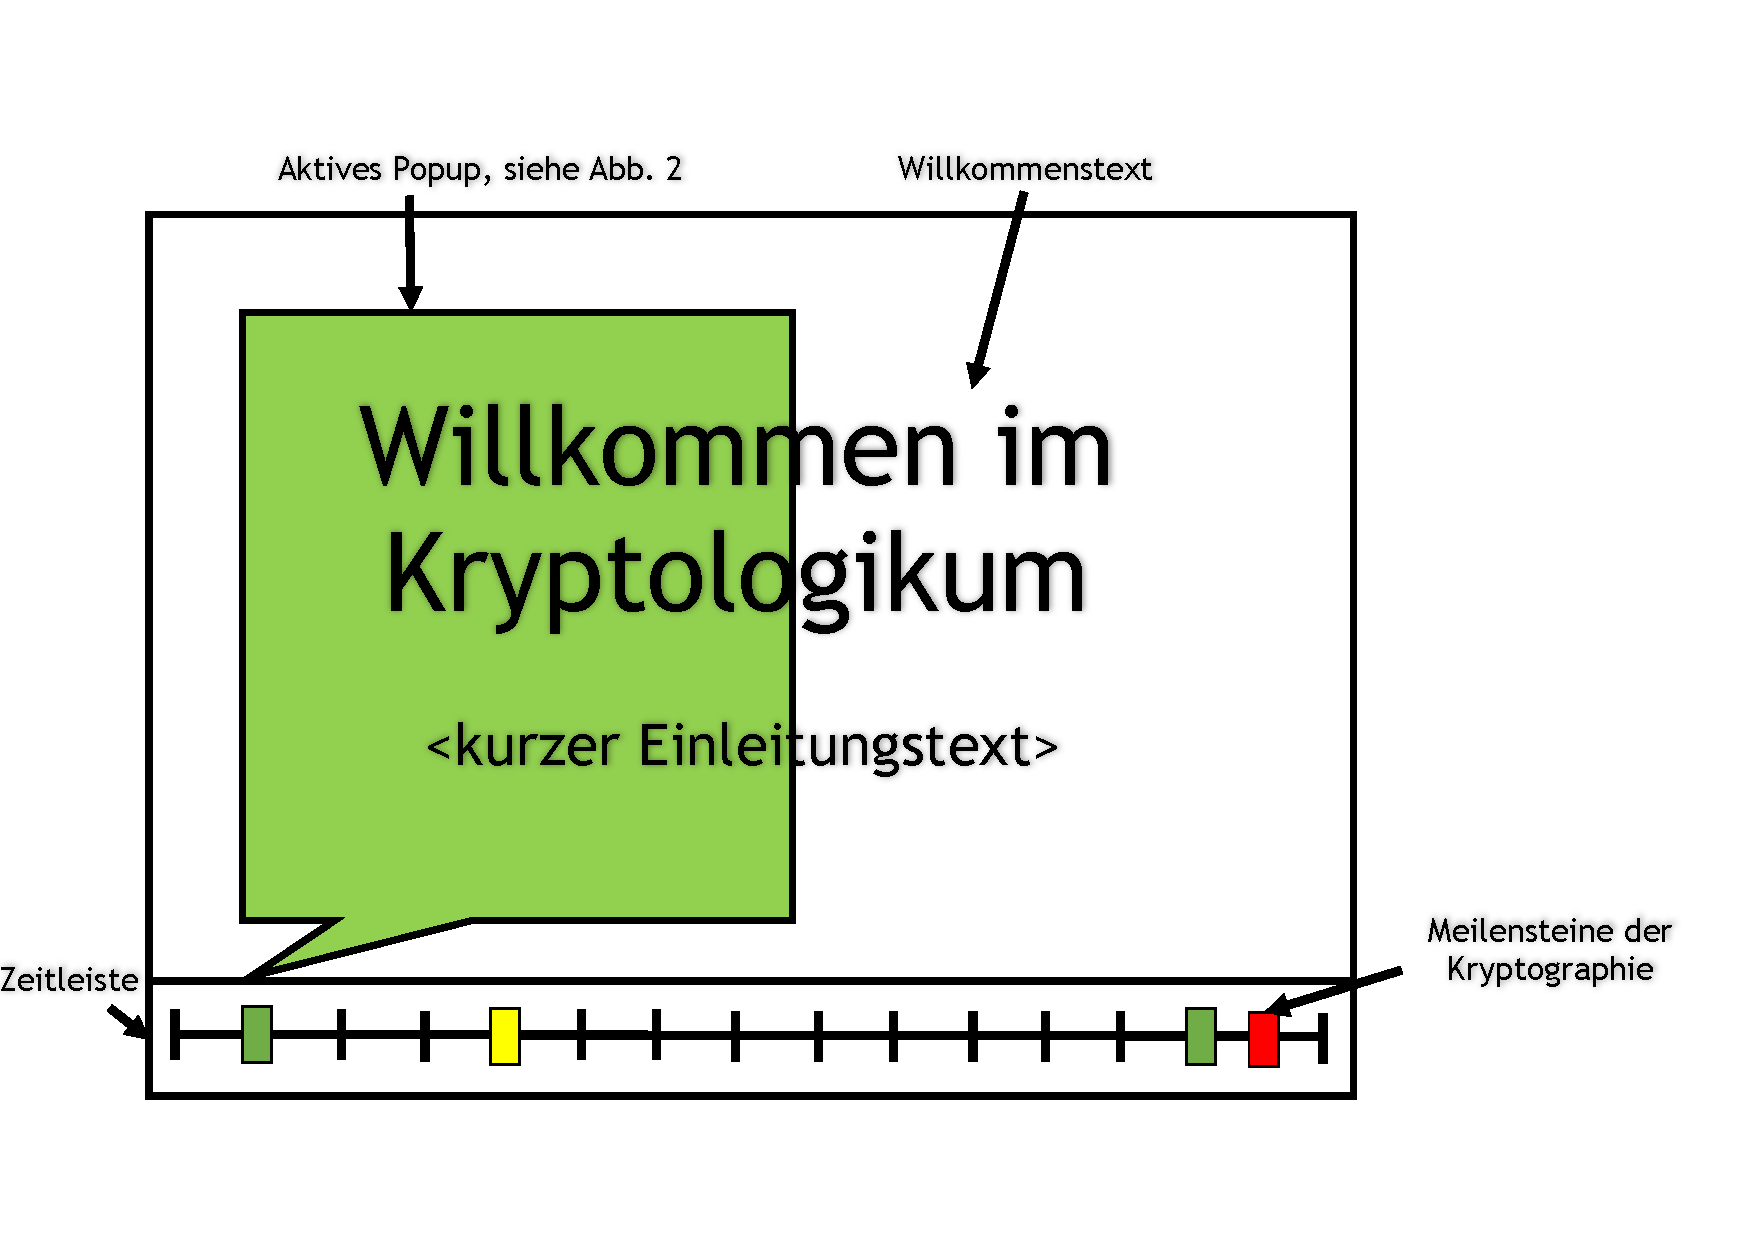
\includegraphics[width=\textwidth]{resources/ui_walkthrough_start-draft}
  \caption{Willkommensbildschirm mit Zeitleiste.}
\end{figure}

Sobald ein Meilenstein ausgewählt wurde, erscheint ein Popover (Fig. 2), dass den Namen, die Schwierigkeit und den Zweck des gewählten kryptografischen Verfahrens noch einmal zusammenfasst. Weiterhin werden ein Screenshot der eigentlichen Visualisierung sowie ein Button, um diese zu starten, dargestellt.

\begin{figure}[H]
  \centering
    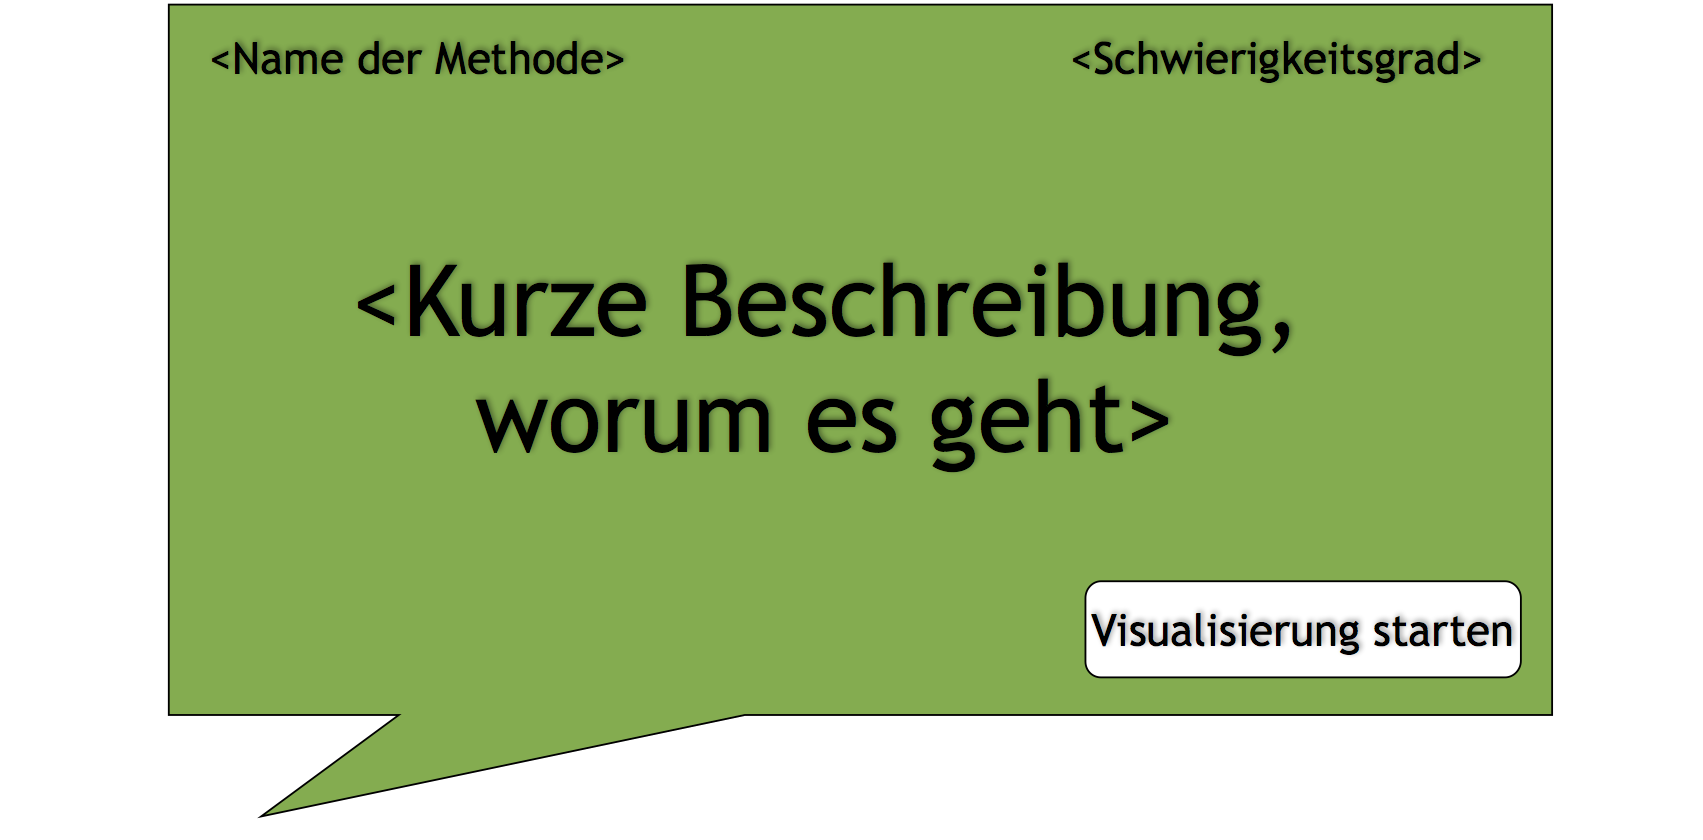
\includegraphics[width=\textwidth]{resources/ui_walkthrough_popover-draft}
  \caption{Detailansicht des Popovers in Fig. 1.}
\end{figure}

Nachdem der Benutzer eine Visualisierung startet, wird diese angezeigt (Fig. 3). Hierbei ist hervorzuheben, dass der Benutzer zu jedem Zeitpunkt die Visualisierung abbrechen kann, indem er auf den Button in der oberen linken Ecke klickt. Hilfe erhält er zu jedem Zeitpunkt im rechten oberen Eck.

\begin{figure}[H]
  \centering
    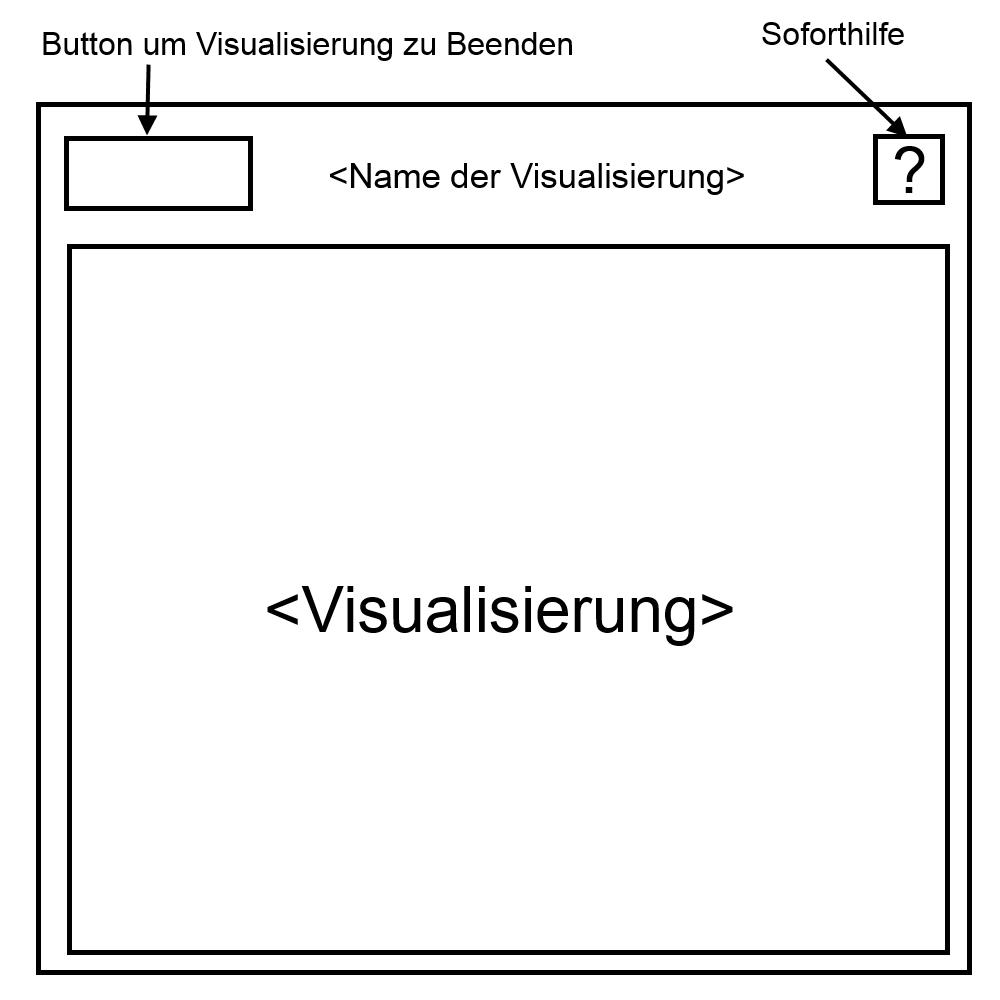
\includegraphics[width=\textwidth]{resources/ui_walkthrough_visualisation-draft}
  \caption{Darstellung einer Visualisierung.}
\end{figure}

Falls der Benutzer die Visualisierung erfolgreich beendet hat, wird (Fig 4.) angezeigt. Zunächst wird dem Benutzer zu seinem Erfolg gratuliert. Weiterhin besteht die prominente Möglichkeit, zum Willkommensbildschirm zurückzukehren. Falls das Interesse des Benutzers geweckt wurde, kann er sich weiterführendes Material mit nach Hause nehmen, indem er den abgebildeten QR-Code scant.

\begin{figure}[H]
  \centering
    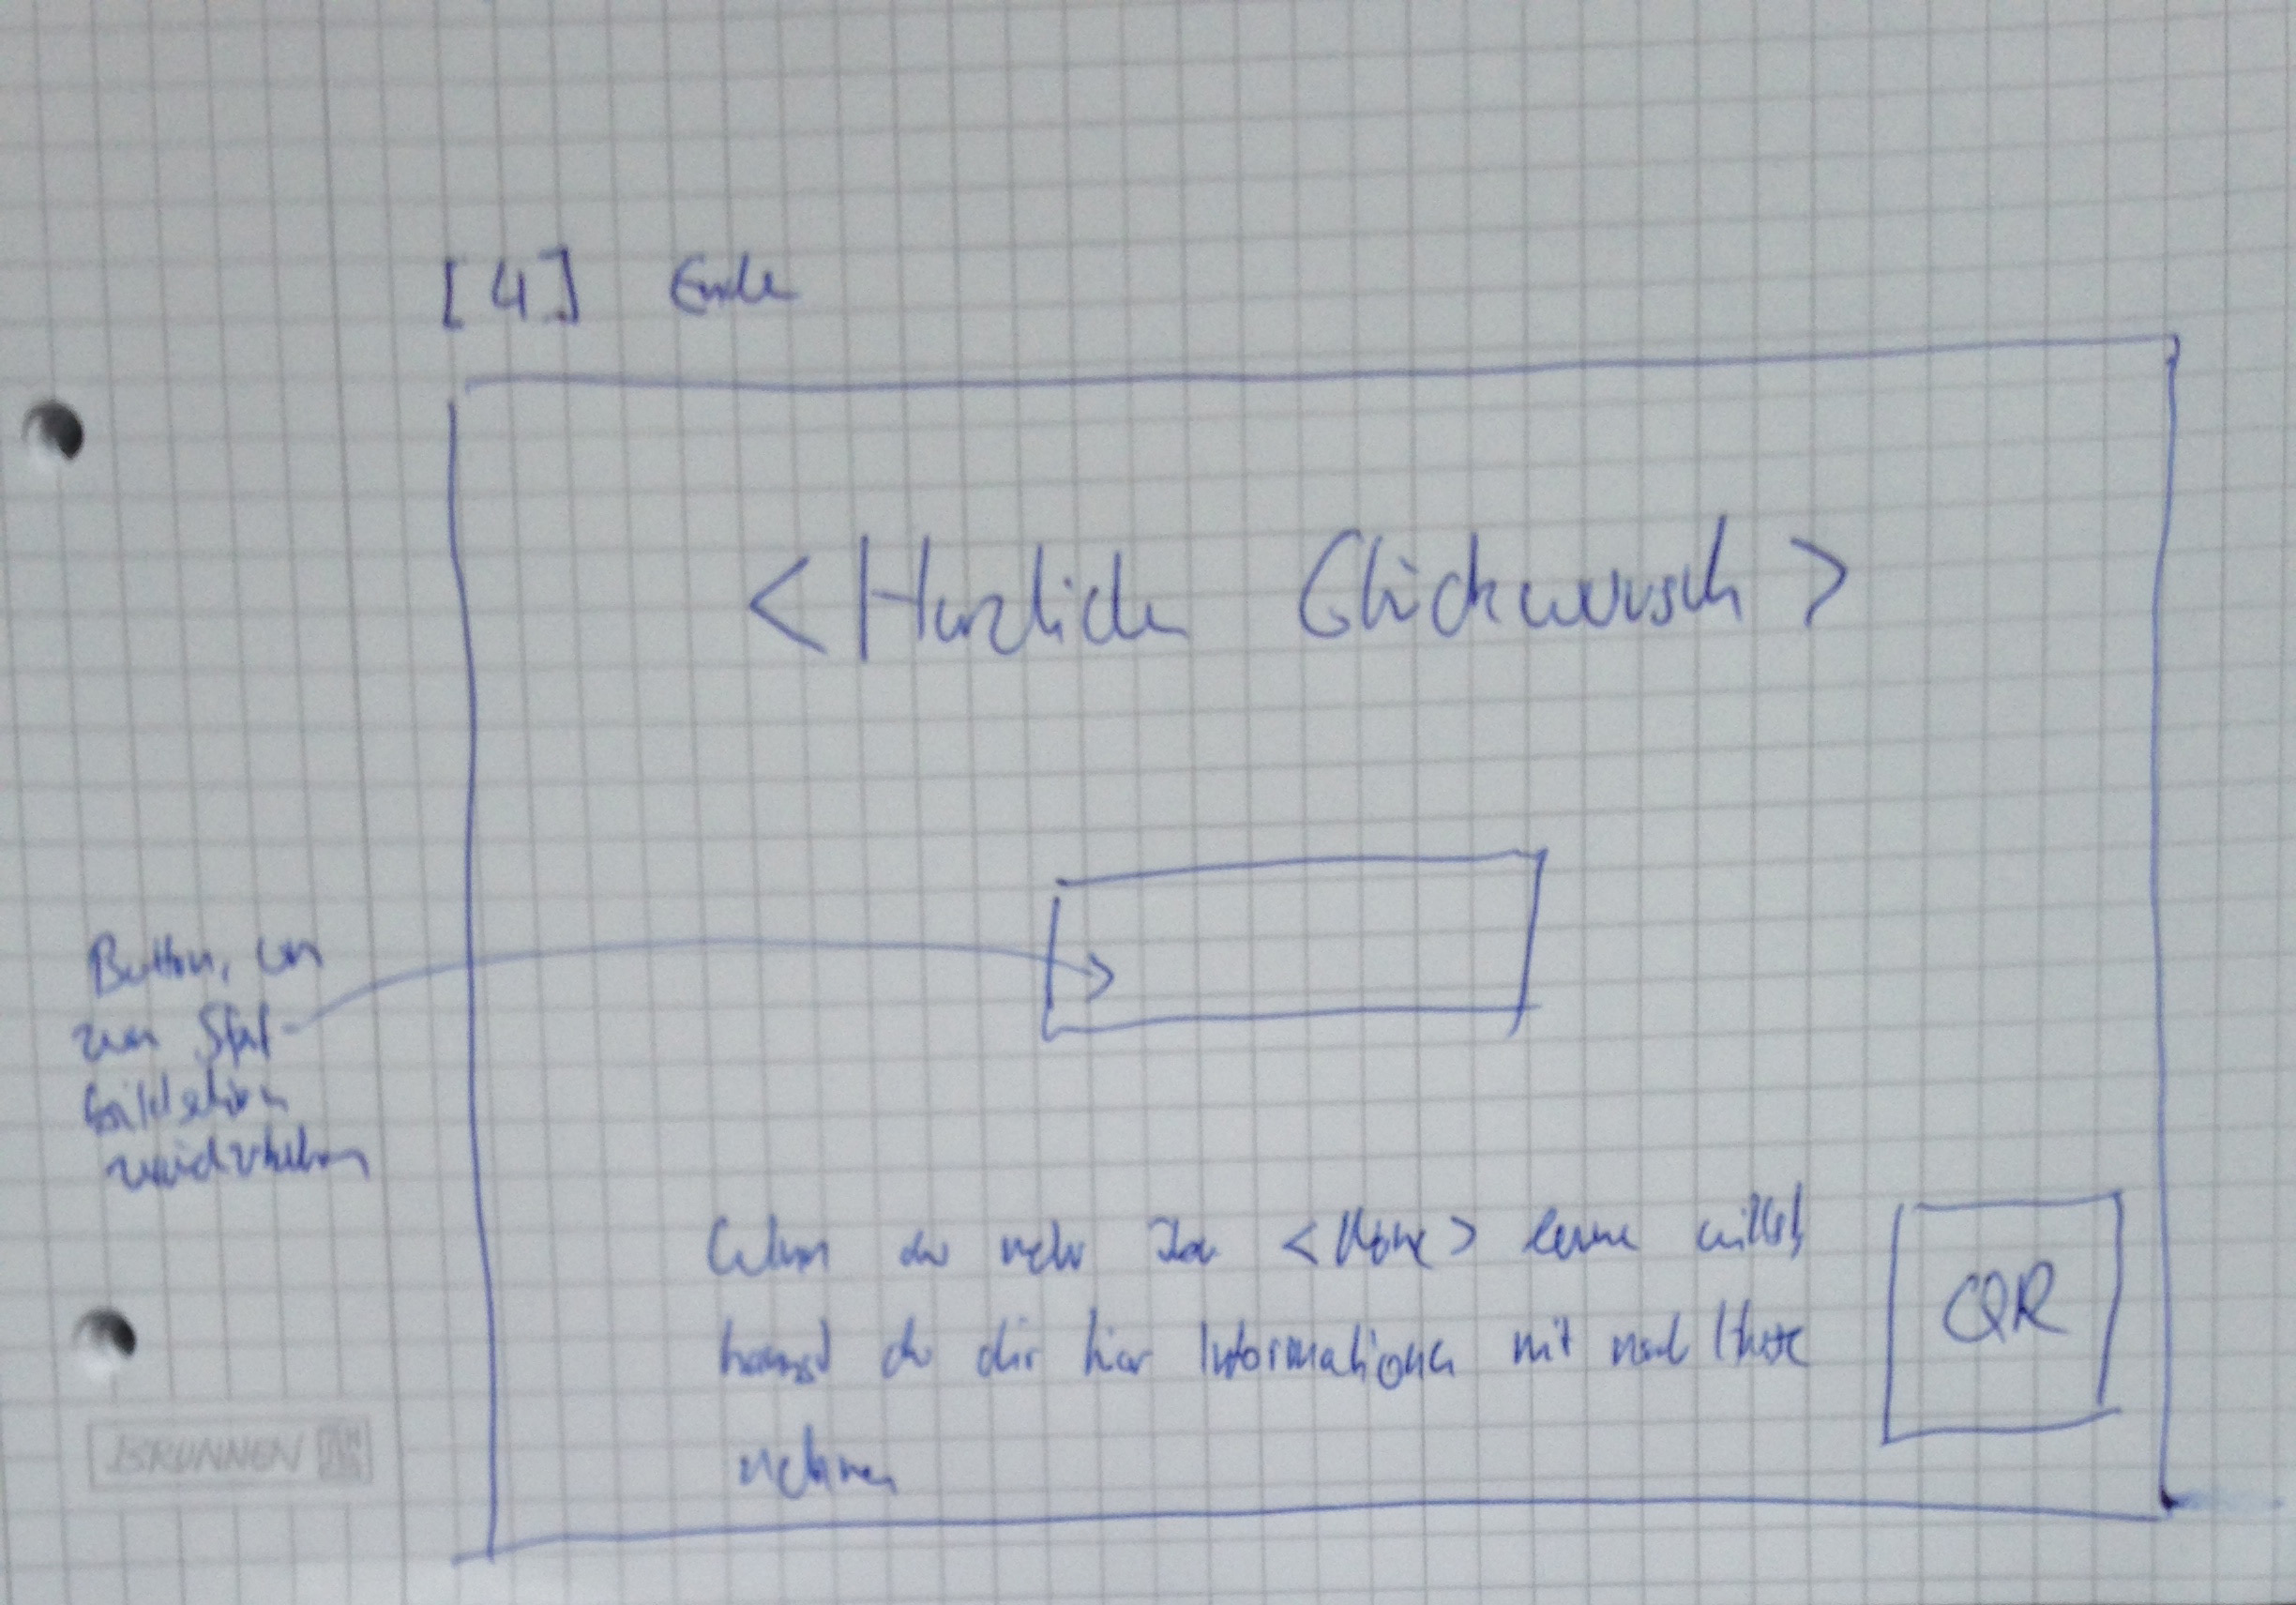
\includegraphics[width=\textwidth]{resources/ui_walkthrough_end-draft}
  \caption{Erfolgreiches Beenden einer Visualisierung.}
\end{figure}


\section{Systemmodelle}

\subsection{Systemübersicht}
Das System verwendet das bekannte MVC-Entwurfsmuster. Weiterhin ist geplant, das System in zwei Schichten zu unterteilen. Von unten nach oben enthält Schicht 1 wiederverendbare und in sich abgeschlossene Bibliotheken. Zum einen handelt es sich hierbei um Code von Dritten (z.B. um QR-Codes zu generieren). Weiterhin ist eine Sammlung wiederverwendbarer Klassen (nachfolgen {\it CGKit} genannt) geplant. {\it CGKit} wird vor allem aus UI-Elemente bestehen, die für die Implementierung aller Visualisierungen wertvoll sind.

\begin{figure}[h!]
  \centering
    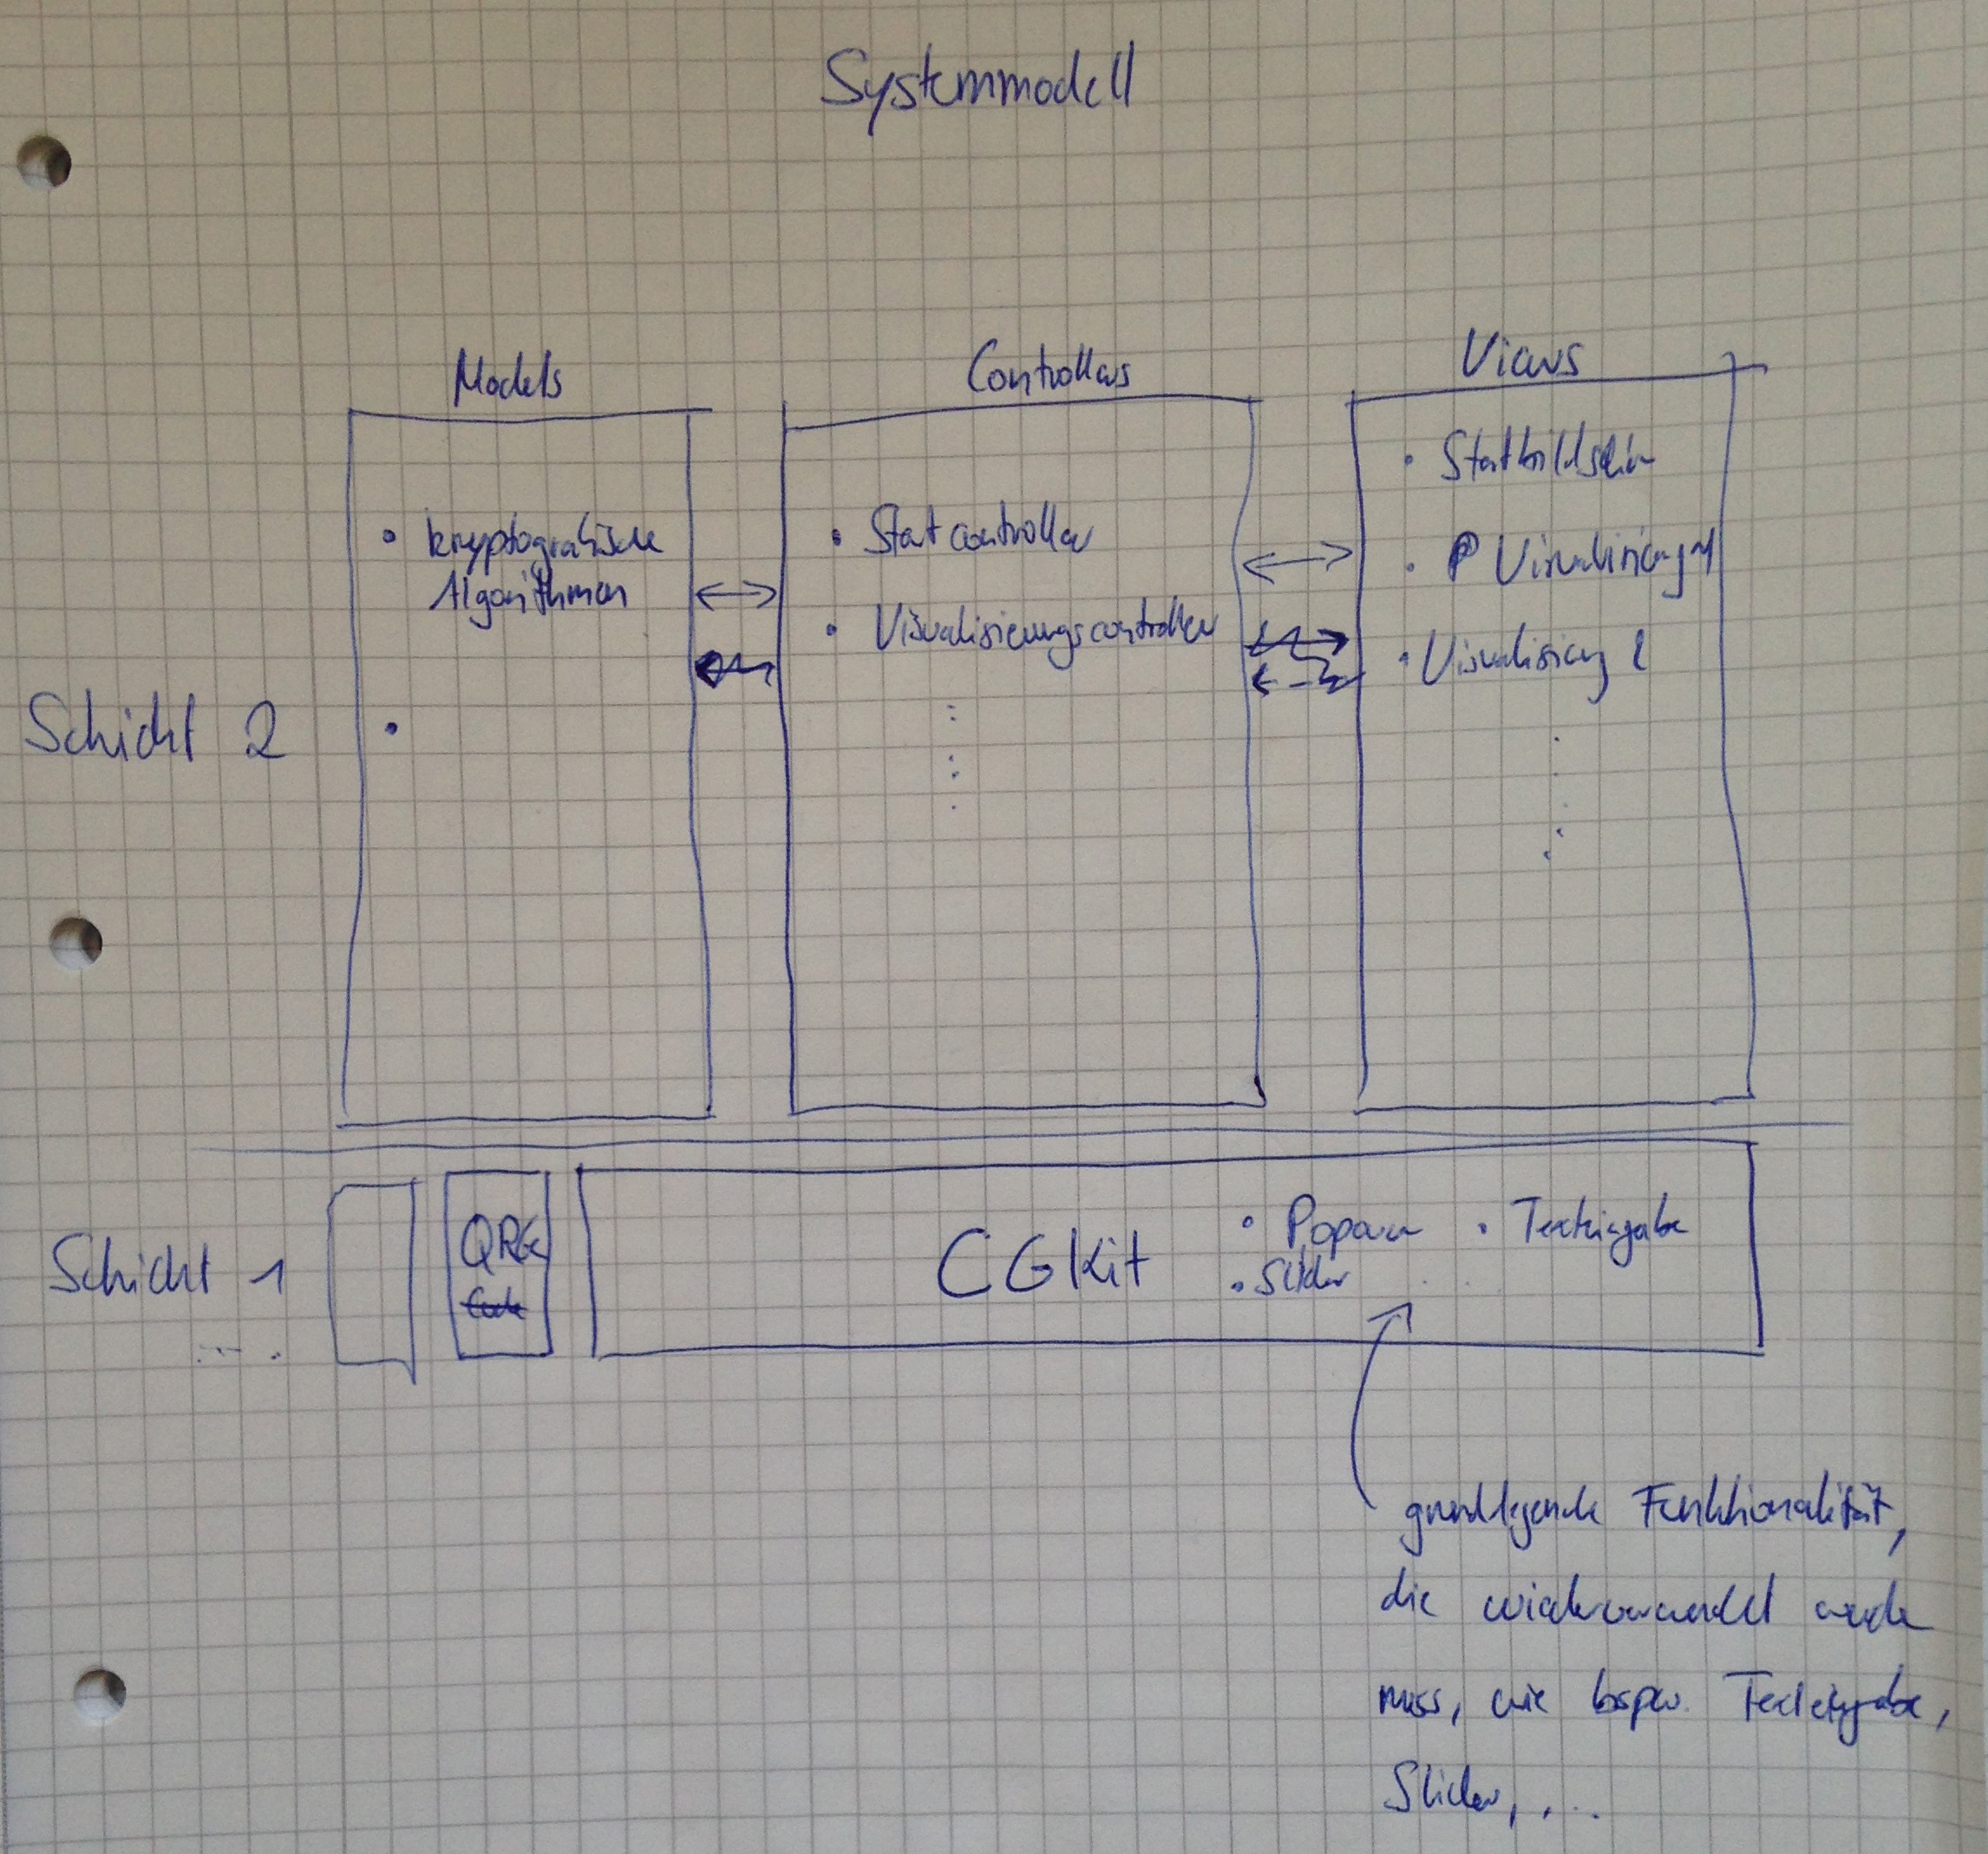
\includegraphics[width=\textwidth]{resources/systemmodel-draft}
  \caption{Schematische Darstellung des beschriebenen Systems.}
\end{figure}

\section{Beispielszenarien}
\begin{itemize}
    \item Beispiel läuft schrittweise ab. Problem wird dargestellt: A möchte B eine Nachricht schicken, die nicht von einer anderen Person als B gelesen werden soll. C versucht die Nachricht zu bekommen. Dabei können A und B nur über ein unsicheres Medium kommunizieren (Analogie z.B. schlüssel per Post verschicken), das von C abgehört wird.
itemA und B generieren ihre Schlüsselpaare. Der genaue Schlüssel ist nicht relevant.
\item A fragt B nach seinem public key, den B auch bereitwillig mitteilt. C hört den public key von B.
\item A verschlüsselt die Nachricht mit dem public key von B und verschickt die Nachricht an B. C hört die verschlüsselte Nachricht ab.
\item B entschlüsselt die Nachricht von A mit seinem private key und kann die Nachricht lesen
\item C versucht mit der Nachricht irgendetwas anzufangen und versucht sie mit dem abgehörten public key von B zu entschlüsseln. Das scheitert natürlich.

Beispiel einer Visualisierung anhand des Caesar-Algos:

\item Es wird erklärt, dass vermutlich Caesar dieses Verfahren verwendet hat um geheime Nachrichten zu verschlüsseln
\item Erklärung des Prinzips an einem Beispielsatz. Es werden schrittweise alle gleichen Buchstaben markiert und in ihr Äquivalent umgewandelt (z.B. "Hallo, wie geht's?" -> zuerst alle H zu K, dann alle a zu d, dann alle l zu o). Hier gibt es die Möglichkeit, schrittweise durchzugehen und noch mal zurück zu gehen. Außerdem kann man wenn man das Prinzip verstanden hat ans Ende springen.
\item Als nächstes muss die Person ein Wort selbst verschlüsseln mit Vorschrift (z.B. a -> b).
\item Am Ende wird mithilfe eines Diagrammes und der Kenntnis, das E der häufigste Buchstabe im Deutschen ist gezeigt, dass man diese Verschlüsselung leicht umgehen kann
\end{itemize}

\textbf{Szenario 1}:
Bob ist interessiert in Kryptographie und besucht zu diesem Anlass das Kryptologikum, um mehr Informationen diesbezüglich zu erhalten. Er nähert sich dem Cryptographics, wo ein Bildschirmschoner verschiedene kryptographische Verfahren Teaser-ähnlich visualisiert. Eine Berührung des Bildschirmes zeigt die Willkommensoberfläche von Cryptographics: Ein Zeitstrahl, auf dem chronologisch angeordnet verschiedene kryptographische Verfahren, ihrem Erfindungsjahr zugeordnet, genannt werden und farblich durch ihre Komplexität von grün (leicht) bis rot (schwer) gekennzeichnet sind. Bob wählt durch eine Berührung die Cäsar-Chiffre aus, sie befindet sich nämlich ganz am Anfang des Zeitstrahls. Daraufhin erscheint eine kurze Einleitung als Popup, im Hintergrund baut sich die Oberfläche auf und der Zeitstrahl gleitet verkleinert als Gesamtübersicht an den unteren Bildschirmrand. Nach dem Durchlesen der Einleitung schließt Bob das Popup, und er sieht eine Demonstration der Cäsar-Chiffre als Schritt-für-Schritt-Beispiel auf einer speziell für das Verfahren ausgelegten Oberfläche. Auf genau dieser Oberfläche kann Bob nach dem Beispiel sein neu erlerntes Wissen über das Verfahren anwenden, um Texte zu verschlüsseln, und durch einen gegebenen Schlüssel zu entschlüsseln. Nachdem er das Verfahren nun verinnerlicht hat, kann Bob das nächste Verfahren auswählen, entweder durch Drücken der “Weiter”-Taste, oder indem er ein Verfahren direkt am Zeitstrahl auswählt. Da er die weiteren Verfahren auch noch sehen möchte, arbeitet er sich am Zeitstrahl entlang durch das Programm, wobei er dann schließlich auf das Diffie-Hellman-Verfahren trifft, über welches er noch mehr Informationen erhalten möchte. Er berührt einen dafür vorgesehenen Button, welcher ein Popup mit einem QR-Code öffnet, dass letztendlich zu den ausführlichen Quellen weiterleitet. Alternativ ist dort auch eine gekürzte URL zu finden die man schnell abschreiben kann (Bsp.: http://goo.gl/abcd12).\\

\textbf{Szenario 2}:
Die ungeduldige Alice wurde von ihrer Freundin überredet, an der Ausstellung teilzunehmen. Sie sieht das Cryptographics und versucht, es durch wiederholte zufällige Eingaben zum Absturz zu bringen. Das Programm zeigt sich jedoch schnell als zu robust, um einem solchen Angriff zu erliegen. Schließlich wählt sie das komplizierteste kryptographische Verfahren aus, um Besuchern nach ihr den Einstieg zu erschweren. Nachdem sie gegangen ist, muss sie jedoch enttäuscht feststellen, dass der nächste Besucher keine weitere Schwierigkeiten hatte, das Programm mit dem dafür vorgesehenen Button in den Grundzustand zurückzuversetzen.\\

\textbf{Szenario 3}:
Nachdem Bob nun längere Zeit an Cryptographics verbracht hat, blickt er erschreckt auf die Uhr um festzustellen, dass es schon viel zu spät geworden ist. Er bricht auf, und lässt das Programm genau so zurück, wie er es gerade eben noch benutzt hat. x Sekunden nach seiner letzten Interaktion erscheint eine Meldung, die Bob darauf hingewiesen hätte, dass sich das Programm bald zurücksetzt, sollte in den nächsten y Sekunden keine Eingabe mehr erfolgen. Da er jedoch schon an der Bushaltestelle steht, aktiviert Cryptographics nun den Bildschirmschoner, den Bob zuvor auch schon vorgefunden hatte, und setzt im Hintergrund das Programm wieder auf den Ursprungszustand zurück.\\

\textbf{Szenario 4}:
Die Ausstellung ist für diesen Tag nun zu Ende, und die Kryptologikum-Administratorin Claudia schließt gerade noch die Tür hinter Bob ab, um sich jetzt den strombetriebenen Exponaten zu widmen. Als sie am Cryptographics ankommt, versucht sie zunächst, irgendwie zum Betriebssystem zurückzukehren, um den PC sicher herunterfahren zu können. Nach kurzer Zeit stellt sie fest, dass das ohne eine zusätzlich eingesteckte Hardware-Tastatur auf keinen Fall möglich ist. Sie holt also eine USB-Tastatur, steckt sie ein, kehrt über den Windows-Taskmanager zum Betriebssystem zurück, fährt den PC herunter und macht die Lichter aus.\\

\begin{figure}[h!]
  \centering
    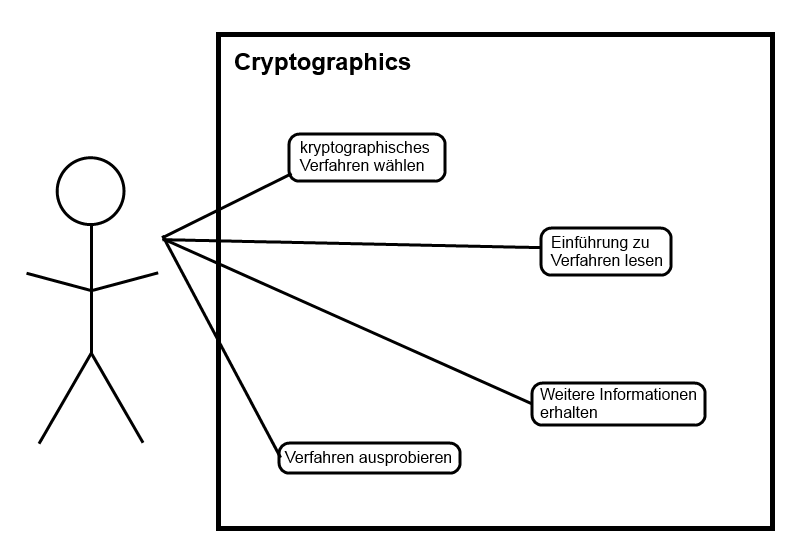
\includegraphics[width=\textwidth]{resources/usecase1}
  \caption{Anwendungsfalldiagramm zu beschriebenen Szenarien.}
\end{figure}

Caesar:
Phase1, Animation:
Startbildschirm von Caesar wird aus einer Animation bestehen, die die Problematik der fehlenden Verschlüsselung in der Römerzeit und die Lösung Caesars erklärt. 
Funktionale Anforderungen für alle Chiffren:(generisch, also auch für Cäsar)
-------------------------------------
Während der Animation ist es jederzeit möglich sofort zum Selbstversuch überzugehen, sowie auch sofortiges wechseln zum textlastigen Geschichtsteil der Chiffre.
Man muss währenddessen jederzeit über die Timeline zum nächsten Verschlüsselungsverfahren wechseln können.
Auch der Teil für Zusatzinformationen, der die QR-Codes enthält, muss erreichbar sein. 
Nachdem die Animation zu Ende ist, wechselt der Bildschirm in die Phase2.
-------------------------------------
Phase2, Selbstversuch:
Man wird anfangs aufgefordert irgendeine !kurze Zeichenkette oder seinen Vornamen einzugeben. Auf der Eingabe wird dann in den nächsten Schritten gearbeitet.
             Der Aufbau des Selbstversuchs gestaltet sich folgendermaßen:
                    In der Mitte des Bildschirms sieht man die Eingabe des Benutzers. Unter der Eingabe ist das Alphabet abgebildet, wobei jeder Buchstabe dort nummeriert ist. Der erste Schritt des Selbstversuchs ist es die Eingabe selbst zu verschlüsseln. Dies geschieht indem jeder Buchstabe der Eingabe nacheinander aufleuchtet und der Benutzer den dazu gehörigen verschlüsselten Buchstaben im Alphabet anklickt. Das Chiffrat taucht zwischen der Eingabe und dem Alphabet auf, sodass unter jedem Buchstaben sein verschlüsseltes Pendant ist. Nachdem alle Buchstaben abgearbeitet sind, entschlüsselt das Programm das Chiffrat selbst und zeigt die Ausgabe unterhalb des Chiffrats an.
                     Der zweite Schritt des Selbstversuchs besteht in der Entschlüsselung eines gegebenen Chiffrats(welcher nicht größer als die Eingabe des Benutzer von vorhin sein soll). Dies geschieht analog zum ersten Schritt. 
Optional(Wunschkriterien): 
                    Dritter Schritt. Dem Benutzer wird die Möglichkeit gegeben ein gegebenes Chiffrat zu knacken. Wobei hier der Klartext nicht mit Cäsar3 verschlüsselt wurde, sondern mit CäsarK. 
 Wenn alles abgearbeitet ist wechselt der Bildschirm in Phase3, dem Hintergrund der Caesar Chiffre. Sprich die geschichtlichen Hintergründe und seine Besonderheit, sowie auch Schwächen.
Phase3, Verfahrensinformationen:
Zu besprechen. Keine Animationen mehr. Mindestens Vor-/Nachteile des Verfahrens und geschichtlicher Hintergrund.
Sollte der Benutzer noch mehr Informationen zu einem Verschlüsselungsverfahren haben möchte, wird er spätestens in dieser Phase besonders auf die "weiterführende" Literatur verwiesen.

Vigenère:
Phase1, Animation:
Die Animation muss jetzt die Problematik der leichten Knackbarkeit der vorherigen Chiffren und Vigenères Lösung dazu zum Ausdruck bringen. Der Benutzer muss aus der Animation klar entnehmen können wer Vigenère war und wie das Verfahren funktioniert.
Generische Anforderung, wie am Anfang bei Cäsar beschrieben.
Phase2, Selbstversuch:
Der Selbstversuch bei Vigenère erfordert für das volle Verständnis eine mindestens doppelt so lange Zeichenkette, wie bei Cäsar, zur Abarbeitung.
Anfangs wird wie bei Cäsar eine Eingabe gefordert, auf der gearbeitet wird. Die Eingabe besteht aus der Zeichenkette die verschlüsselt wird und aus dem Schlüssel(Codewort).
Die Schrittreihenfolge ist wie bei Cäsar. Zuerst muss der Benutzer die Eingabe mit dem eingegeben Codewort verschlüsseln und im zweiten Schritt dann ein vorgegebenes Chiffrat mit einem vorgegebenen Schlüssel entschlüsseln.
Das Verschlüsseln wird folgendermaßen in Szene gesetzt:
           Die Eingabe des Benutzers wird zentral auf dem Bildschirm angezeigt. Unterhalb ist wieder das Alphabet mit drunter liegender Nummernfolge abgebildet. Unterhalb des Codewortes bekommt jeder Buchstabe seine Nummer aus dem Alphabet, sodass der User weiß um wie vielen Stellen das Klartextzeichen zu verschieben ist. Verschlüsselt wird indem jeder Buchstabe der Eingabe und des Codeworts nacheinander aufleuchtet und der Benutzer das dazu gehörige Chiffrezeichen im Alphabet anklickt. Unter der Eingabe wird anschließend das Chiffrat abgebildet und das Programm entschlüsselt am Ende das Chiffrat und zeigt das Ergebnis an.
Entschlüsselt wird analog. Hier sind aber das Chiffrat und Codewort vorgegeben. Das Ergebnis wird anschließend unter dem Chiffrat angezeigt.
Optional:
Dritter Schritt. Dem Benutzer wird die Möglichkeit gegeben ein gegebenes Chiffrat ohne des Codewortes zu entschlüsseln. Benötigte Hilfsmittel, wie die Häufigkeitsanalyse sind bereit zu stellen. Muss jedoch ebenfalls noch abgeklärt werden, wie genau, da auf zu kurzen Zeichenketten die Häufigkeitsanalyse wie bei Cäsar zu wenig Aussagekraft.
Phase3 ist analog wie bei Cäsar.

Public Key Infrastruktur(PKI):
Eins vorneweg: Da dies eine aktuelle Problematik ist, ist es wichtig die Animationen anhand von aktuellen Beispielen aus dem heutigem Alltag darzustellen.
Phase1, Animation:
Es ist Anhand einer Animation zu zeigen, wie die Authentifikation öffentlicher Schlüssel mithilfe von Zertifikaten realisiert wird. Es muss daraus ersichtlich sein, wie die Zertifikate beweisen, dass der öffentliche Schlüssel zum anderen Kommunikationspartner gehört und nicht durch einen Angreifer ausgetauscht wurde. 
Vorausgesetzt man hat die Grundlagen über public key Kryptographie und Hashing verinnerlicht ist dieses System unter die Schwierigkeit "Mittel" einzuordnen. Es ist jedoch auch möglich die Schwierigkeit zu reduzieren indem man die Signaturen bspw. durch eine einfache Unterschrift ersetzt, das beispielhaft für eine Signatur stehen kann. So kann die Schwierigkeit auf "Einfach" zu reduziert werden.
Es ist jedoch zu beachten, dass hierzu mehrere Animationen notwendig sind um die PKI, wie sie heute eingesetzt ganz verstehen können. Dies liegt daran, dass verschieden Vertrauensmodelle benutzt werden. Zuallererst ist die Rollenvielfalt auf einen User und Certification Authority(CA) zu beschränken. User will in diesem Fall seinen öffentlichen Schlüssel von der CA signieren lassen, sodass bei der Kommunikation mit anderen Usern er neben seinem Schlüssel auch ein Zertifikat vorlegen kann, dass der Schlüssel nicht verändert wurde und er dazu den passenden secret key besitzt. So weiß der andere Kommunikationspartner, dass nur der User die, mit dem erhaltenen public key verschlüsselten, Nachrichten entschlüsseln kann. Diese Zertifikate setzen ein gewisses Vertrauen in den Herausgeber(CA) voraus. Denn, wenn die CA nicht wirklich seriös ist, ist das Zertifikat nicht wirklich ein Beweis dafür, dass der Schlüssel nicht verändert wurde. Vertraut man der CA jedoch fest, so ist man dann auch davon überzeugt, dass man die vertraulichen Nachrichten mit dem PK verschlüsseln und abschicken kann. Das führt auf eine weitere Grundlage der PKI, die Vertrauensmodelle. Aufgrund der großen Vielfalt ist hier auch dringend nötig, wie bei der Rollenvielfalt, auf das wichtigste zu reduzieren.
Das erste Modell besteht aus einer oder mehreren CA's, die Zertifikate an Benutzer herausgeben können. Hierzu ist die Problematik aufzuzeigen, die dabei entsteht.
Das zweite ist eine Hierarchie von CA's. Sprich die CA's können andere Benutzer dazu ermächtigen an andere Zertifikate auszustellen. Das Vertrauen in die CA's überträgt sich also auf diesen Benutzer! Was jedoch auch gewisse Probleme mit sich bringt.
Das dritte Modell heißt Anarchie oder auch Web of Trust. Hier ist jeder Benutzer eine CA und kann seine öffentlichen Schlüssel selbst signieren. Wie auch davor bringt das Probleme und Vorteile mit sich.
Phase2, Selbstversuch:
Ist noch zu klären :D
Phase3, Informationen:
Hierzu kann man die geschichtliche Einordnung der Problematik der Schlüsselverteilung der Public Key Kryptosystemen(PKK) aufzuzeigen. Die Akteure, die bei der Entwicklung mitgewirkt haben sind aufzuzeigen. Und weiterer Schnickschnack, der uns noch im Laufe einfällt. Dies Das Ananas.


\section{Globale Testfälle}
- automatisiertes Testen mithilfe von JUnit vor allem der Krypto-Algorithmen
- ggf. automatisiertes Testen der UI mithilfe von Szenarien und geeignetem Framework
Stresstest mit möglichst zufälligen und willkürlichen Eingaben (wie es Kinder eben tun)
Usability Tests mit passenden Testpersonen\\
Es ist sehr ratsam, dass die globalen Testfälle mit /Txy/ sich auf die Funktionalität /Fxy/ beziehen. So ist eine gewisse Konsistenz, Überdeckungsgrad und Übersichtlichkeit gewährleistet. Folgt demnächst, wenn die Funktionalen Anforderungen fertig sind!

\section{Qualitätsbestimmung}

\end{document}


